\subsection{Universal Adversarial Perturbation}
In diesem Kapitel werden die generierten \acrlong{uap}s vor der \Gls{robustifizierung} für jedes der untersuchten Klassifikationsmodelle präsentiert. Diese Modelle wurden jeweils auf den Datensätzen COVIDx CXR-4 und MRI vortrainiert. Es werden ausschliesslich die als relevant erachteten \acrshort{uap}s visualisiert. Weitere \acrshort{uap}s sind im Anhang zu finden. Die Darstellung der \acrshort{uap}s erfolgt in Form von Heatmaps. In diesen Visualisierungen repräsentieren rote Bereiche positive Werte, während blaue Bereiche negative Werte darstellen. Positive Werte führen zu einer Erhöhung des Pixelwertes im Eingabebild, was in einer Aufhellung resultiert, wohingegen negative Werte den Pixelwert reduzieren und folglich zu einer Verdunkelung führen. Graue Werte weisen darauf hin, dass die Perturbationen in diesem Bildbereich keine Änderungen verursachen.

% UAP Resultate
\begin{figure}[H]
    \centering
    \text{\acrshort{uap} von vortrainierten Klassifikationsmodellen auf den MRI Datensatz} \\
    \begin{subfigure}{0.16\linewidth} % Adjust the width to fit six images in one line
        \centering
        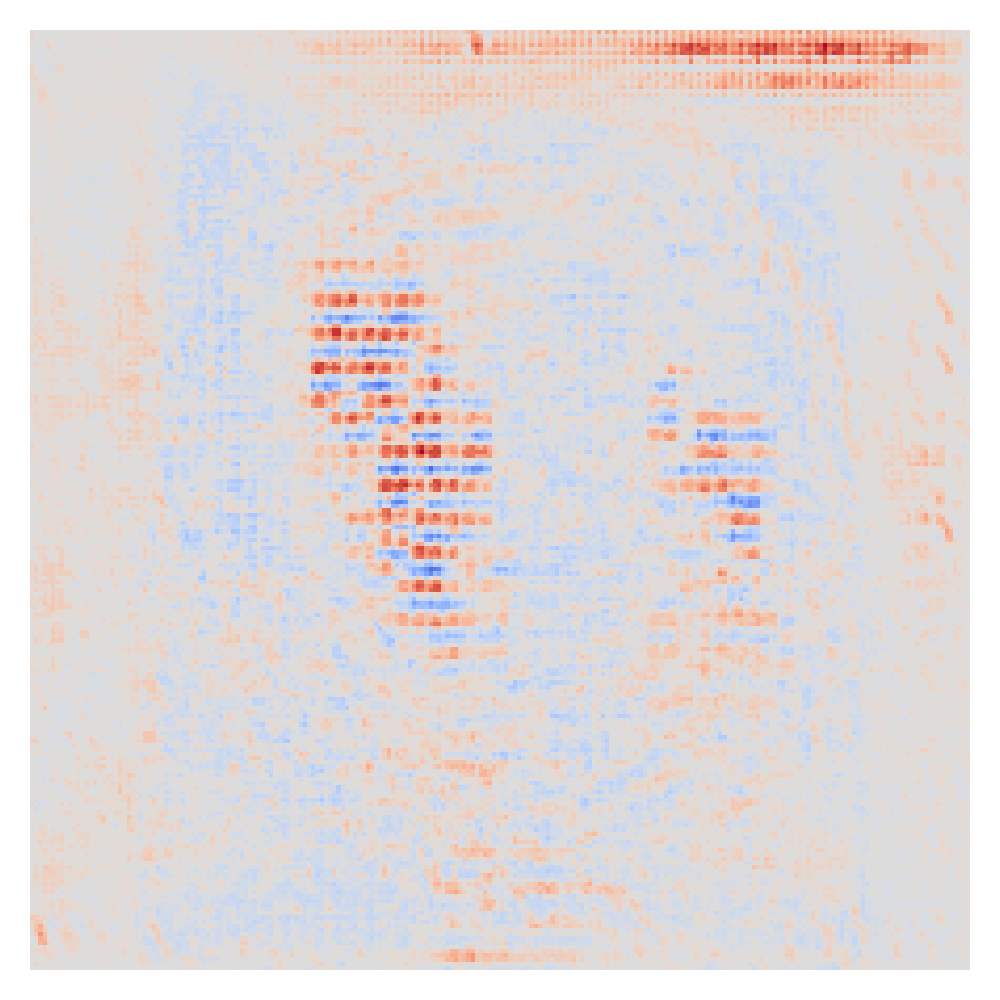
\includegraphics[height=1\linewidth]{01-images/05-resultate/uap_densenet121/uap0-densenet121-mri_data-n200-robustificationslevel0.png}
        \caption{DenseNet121\\\textcolor{white}{Pikachu}}
        \label{fig:uap-densenet121-mri-prerobustification}
    \end{subfigure}\hfill%
    \begin{subfigure}{0.16\linewidth}
        \centering
        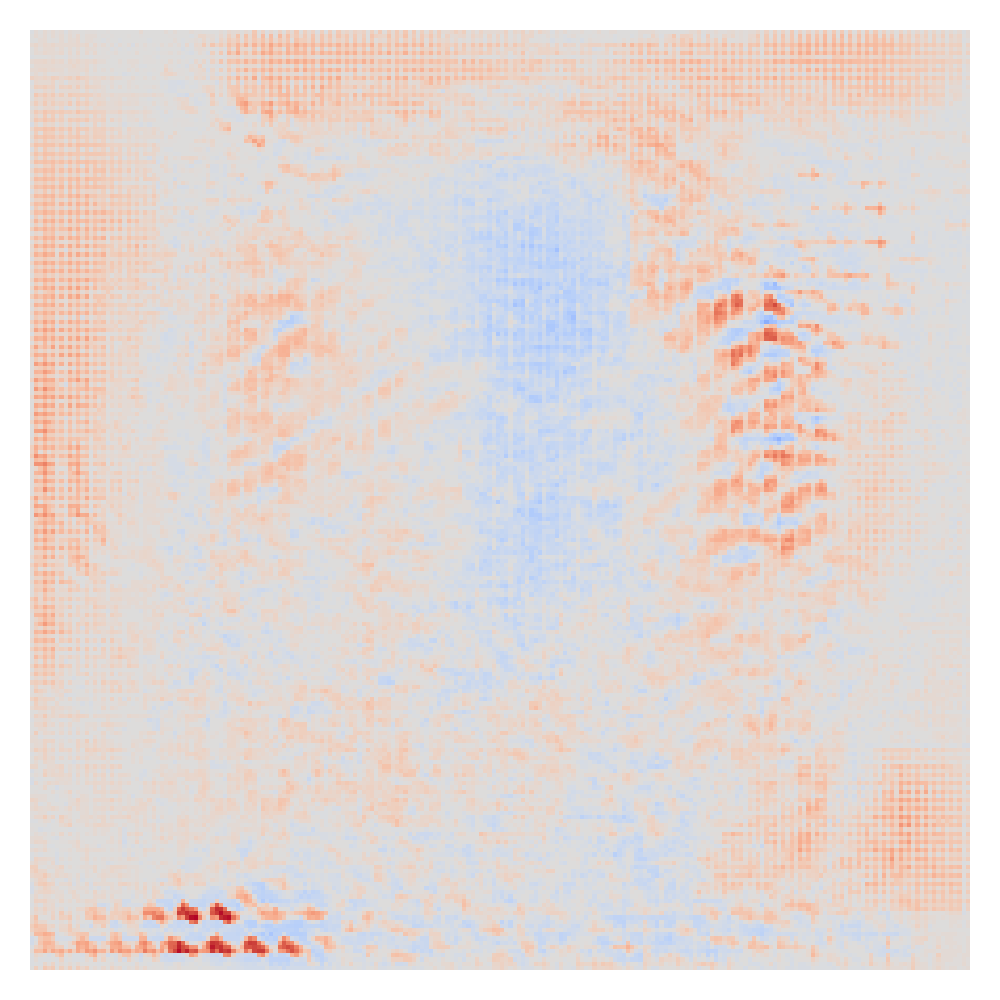
\includegraphics[height=1\linewidth]{01-images/05-resultate/uap_densenet169/uap0-densenet169-mri_data-n200-robustificationslevel0.png}
        \caption{DenseNet169\\\textcolor{white}{Raichu}}
    \end{subfigure}\hfill%
    \begin{subfigure}{0.16\linewidth}
        \centering
        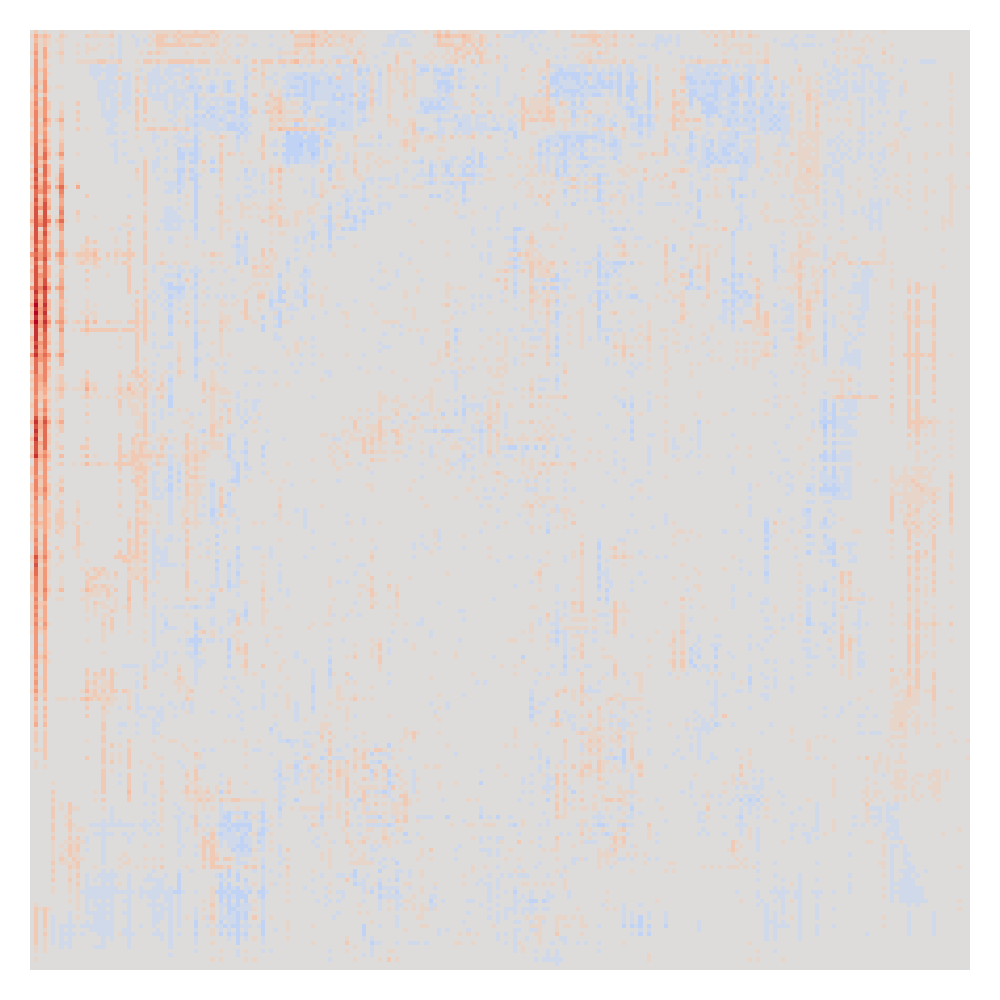
\includegraphics[height=1\linewidth]{01-images/05-resultate/uap_efficientnet_s/uap0-efficientnet_v2_s-mri_data-n200-robustificationslevel0.png}
        \caption{Efficient\\NetV2-S}
    \end{subfigure}\hfill%
    \begin{subfigure}{0.16\linewidth}
        \centering
        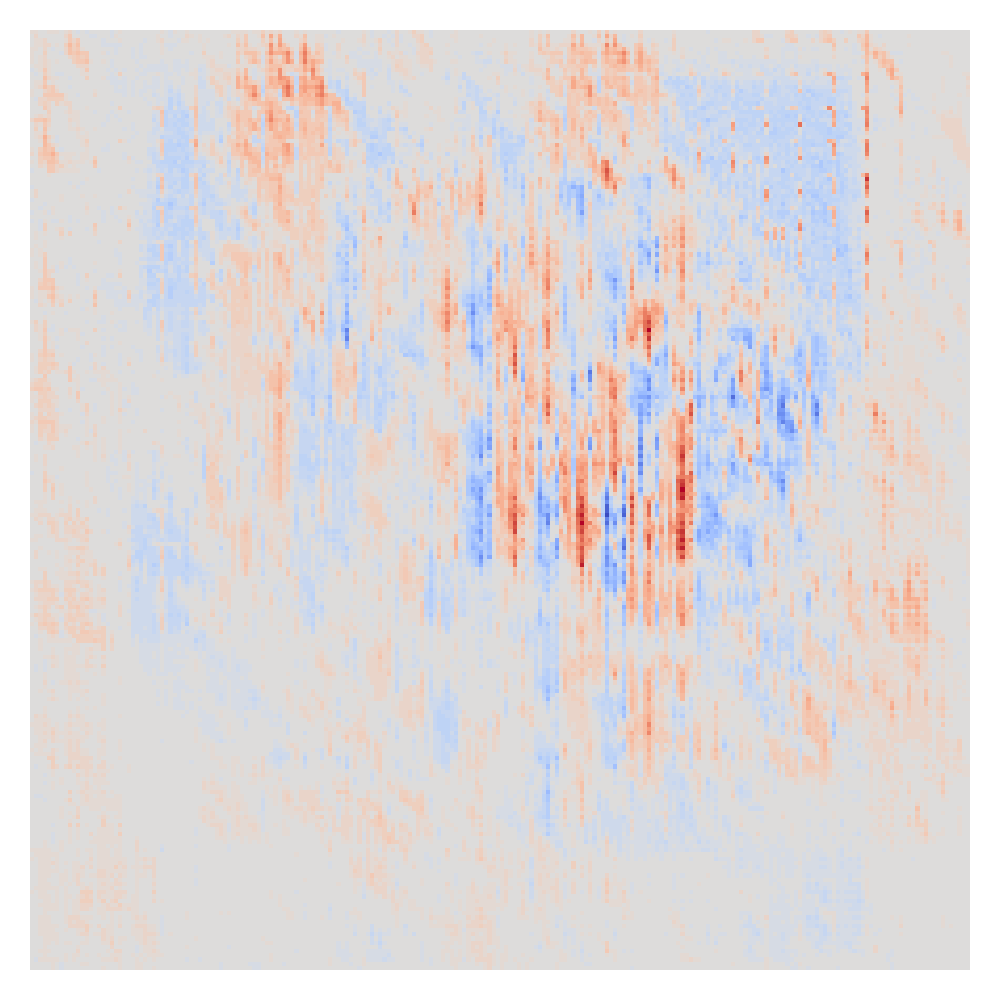
\includegraphics[height=1\linewidth]{01-images/05-resultate/uap_efficientnet_m/uap0-efficientnet_v2_m-mri_data-n200-robustificationslevel0.png}
        \caption{Efficient-\\NetV2-M}
    \end{subfigure}\hfill%
    \begin{subfigure}{0.16\linewidth}
        \centering
        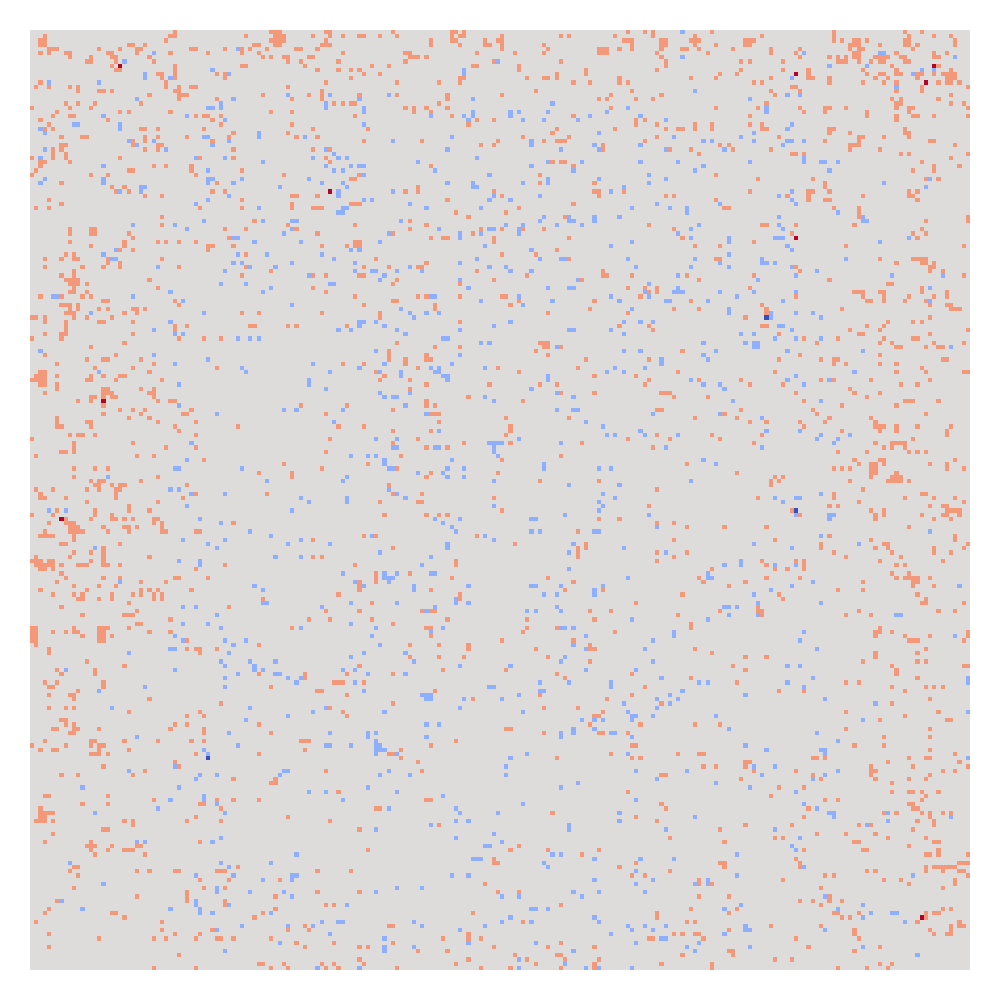
\includegraphics[height=1\linewidth]{01-images/05-resultate/uap_resnet18/uap0-resnet18-mri_data-n200-robustificationslevel0.png}
        \caption{ResNet18\\\textcolor{white}{6er incoming}}
    \end{subfigure}\hfill%
    \begin{subfigure}{0.16\linewidth}
        \centering
        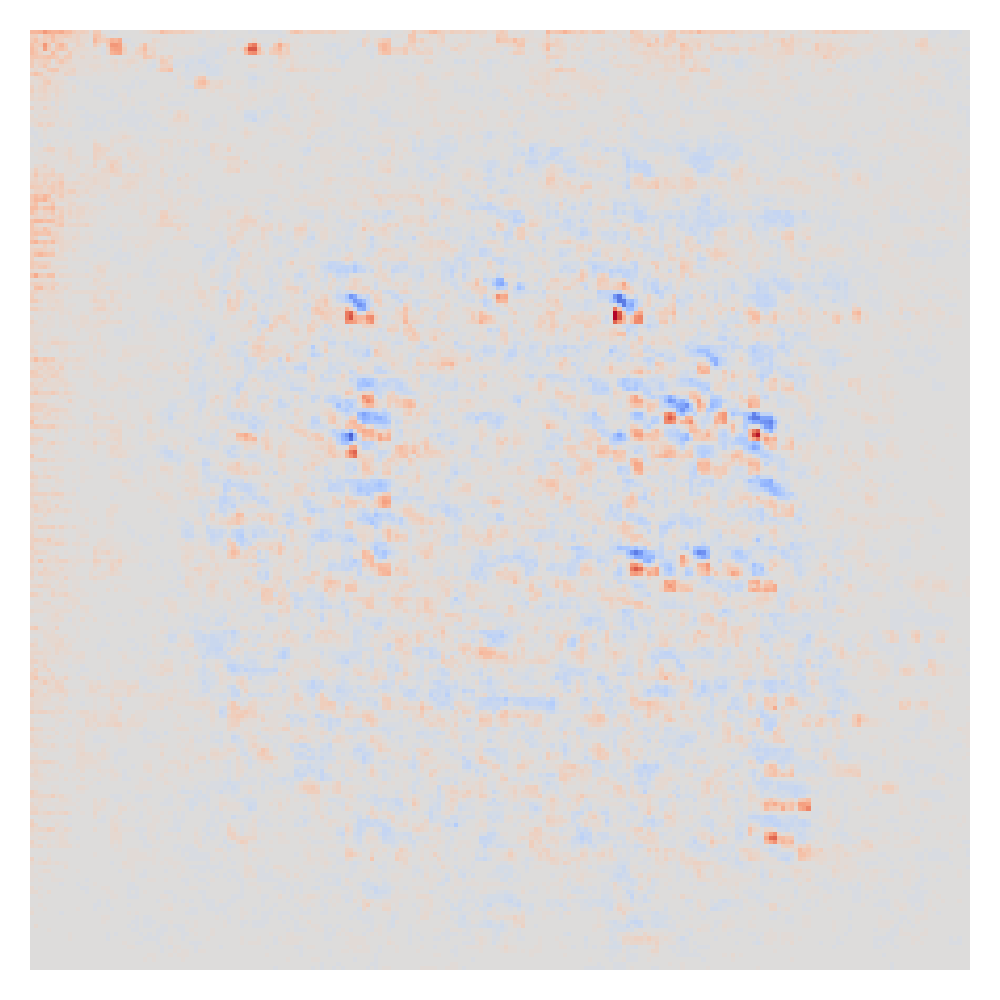
\includegraphics[height=1\linewidth]{01-images/05-resultate/uap_resnet50/uap0-resnet50-mri_data-n200-robustificationslevel0.png}
        \caption{ResNet50\\\textcolor{white}{messi goat}}
    \end{subfigure}
    \caption{Darstellung generierter \acrshort{uap}s für den Hirntumor-Datensatz, basierend auf 200 Trainingsbildern und verschiedenen Klassifikationsmodellen.}
    \label{fig:unterschiedliche-uaps-mri}
\end{figure}

In den \acrshort{uap}s in Abbildung \ref{fig:unterschiedliche-uaps-mri} sind spezifische Muster erkennbar, die charakteristisch für jedes Modell sind. 

Die \acrlong{uap} für DenseNet121 zeigt in der Heatmap eine klare Struktur mit horizontalen, alternierenden Mustern. Im Zentrum sind blaue Bereiche zu sehen, während die Ränder überwiegend rote Muster aufweisen. Diese Verteilung deutet darauf hin, dass die \acrshort{uap} in diesen Regionen besonders effektiv ist. Bei DenseNet169 hingegen dominiert ein grosser blauer Bereich das Zentrum, umgeben von zahlreichen roten Flecken, die sich über das gesamte Bild erstrecken.

EfficientNetV2-S zeigt insgesamt sehr feine Perturbationen, wobei die linke Seite durch eine deutliche rote vertikale Linie am Rand hervorsticht. Im Gegensatz dazu sind die Perturbationen beim grösseren Modell, EfficientNetV2-M, deutlicher ausgeprägt und weniger fein granular. Die Perturbationen in diesem Modell weisen sowohl rote als auch blaue Muster auf, die überwiegend senkrecht verlaufen. Dies ist besonders interessant, da bei der \acrshort{uap} von DenseNet121 horizontale Muster beobachtet wurden.

Bei ResNet18 sind die Perturbationen punktuell, mit roten Bereichen ausserhalb des Zentrums der Heatmap, während im Zentrum tendenziell blaue Werte vorhanden sind. ResNet50 weist ein ähnliches Muster auf, unterscheidet sich jedoch dabei, dass im Zentrum der Heatmap punktuell hohe Perturbationswerte zu beobachten sind. Diese Ausprägungen fehlen in den äusseren Bereichen.

\begin{figure}[H]
    \centering
    \text{\acrshort{uap} von COVIDx CXR-4 trainierten Klassifikationsmodelle} \\
    \begin{subfigure}{0.16\linewidth} % Adjust the width to fit six images in one line
        \centering
        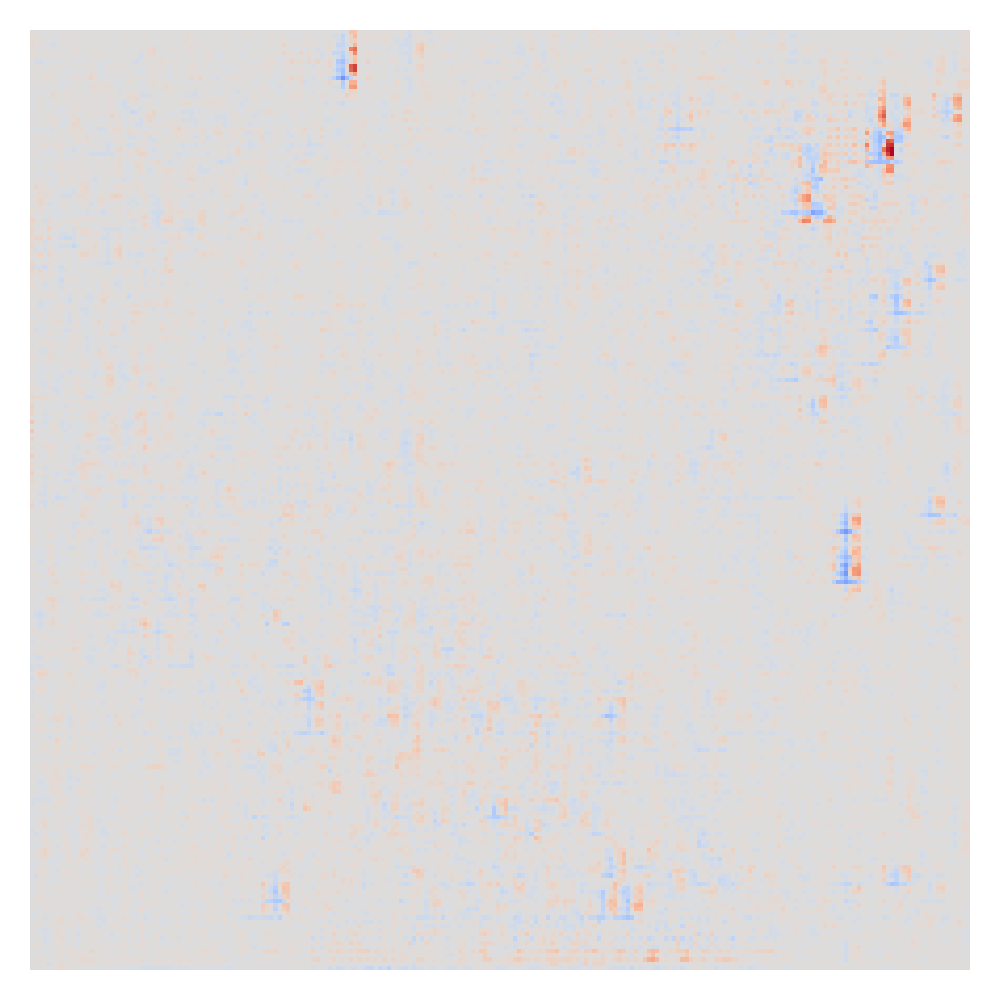
\includegraphics[height=1\linewidth]{01-images/05-resultate/uap_densenet121/uap0-densenet121-covidx_data-n200-robustificationslevel0.png}
        \caption{DenseNet121\\\textcolor{white}{Chandelure}}
    \end{subfigure}\hfill%
    \begin{subfigure}{0.16\linewidth}
        \centering
        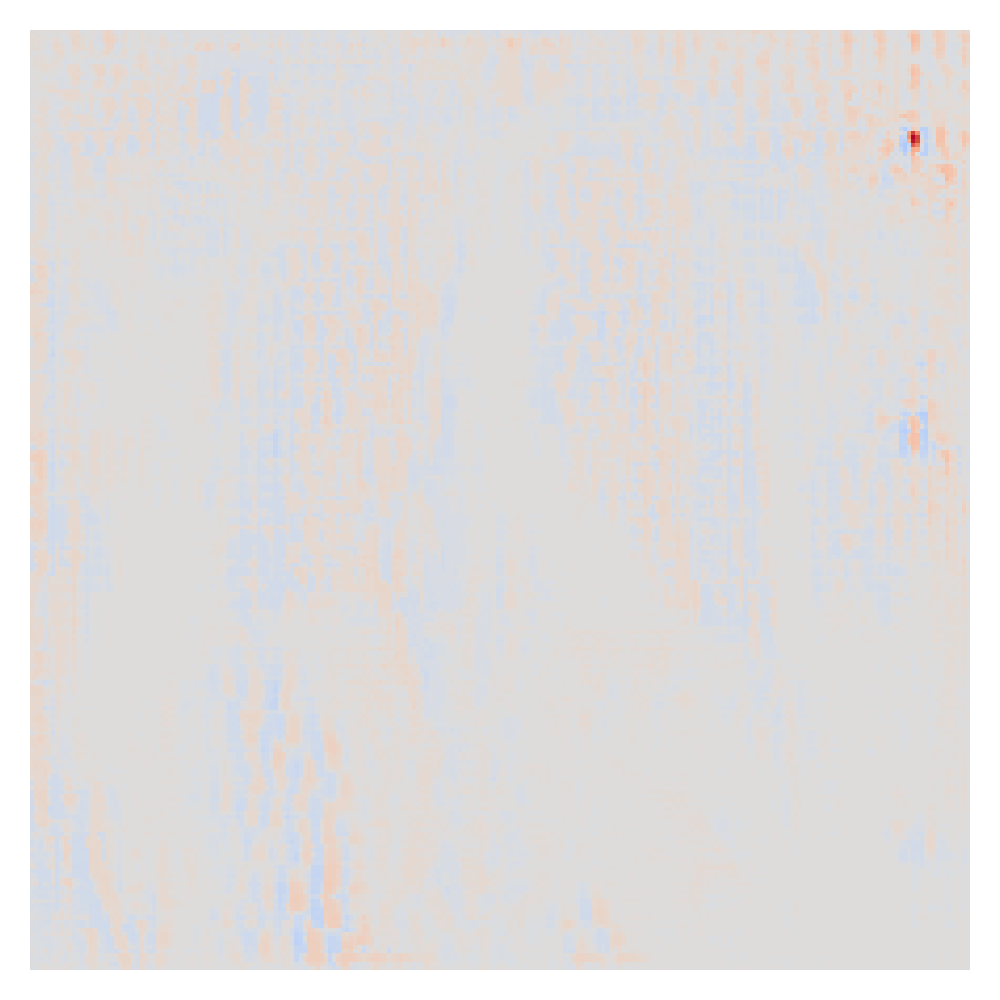
\includegraphics[height=1\linewidth]{01-images/05-resultate/uap_densenet169/uap0-densenet169-covidx_data-n200-robustificationslevel0.png}
        \caption{DenseNet169\\\textcolor{white}{Latias}}
    \end{subfigure}\hfill%
    \begin{subfigure}{0.16\linewidth}
        \centering
        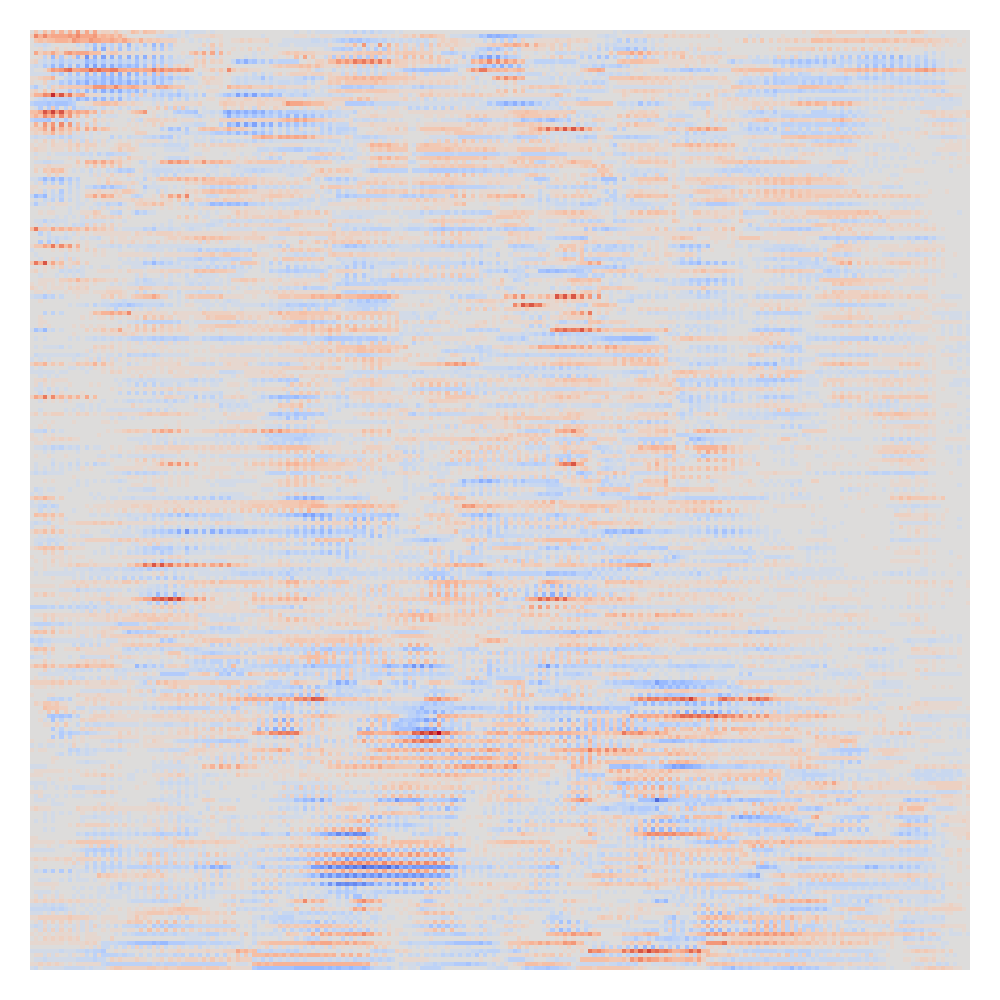
\includegraphics[height=1\linewidth]{01-images/05-resultate/uap_efficientnet_s/uap0-efficientnet_v2_s-covidx_data-n200-robustificationslevel0.png}
        \caption{Efficient-\\NetV2-S}
    \end{subfigure}\hfill%
    \begin{subfigure}{0.16\linewidth}
        \centering
        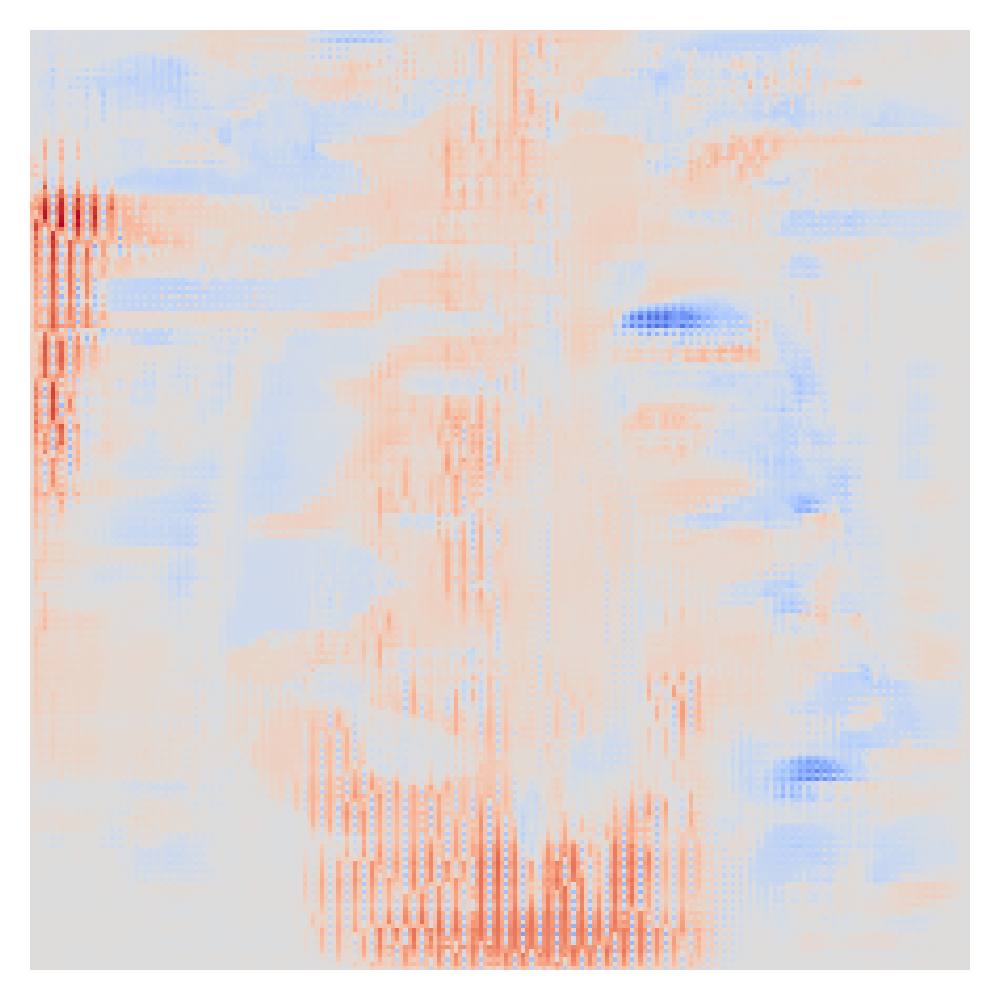
\includegraphics[height=1\linewidth]{01-images/05-resultate/uap_efficientnet_m/uap0-efficientnet_v2_m-covidx_data-n200-robustificationslevel0.png}
        \caption{Efficient-\\NetV2-M}
    \end{subfigure}\hfill%
    \begin{subfigure}{0.16\linewidth}
        \centering
        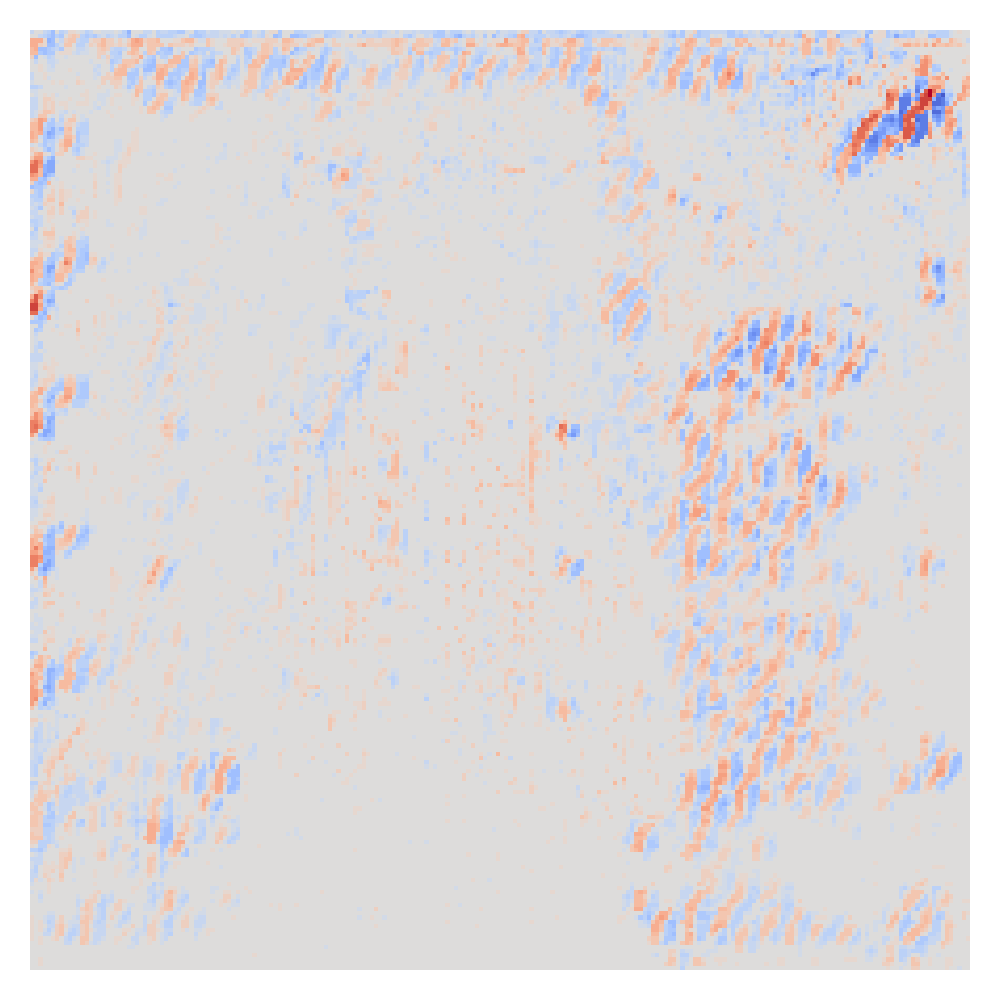
\includegraphics[height=1\linewidth]{01-images/05-resultate/uap_resnet18/uap0-resnet18-covidx_data-n200-robustificationslevel0.png}
        \caption{ResNet18\\\textcolor{white}{Rameidon}}
    \end{subfigure}\hfill%
    \begin{subfigure}{0.16\linewidth}
        \centering
        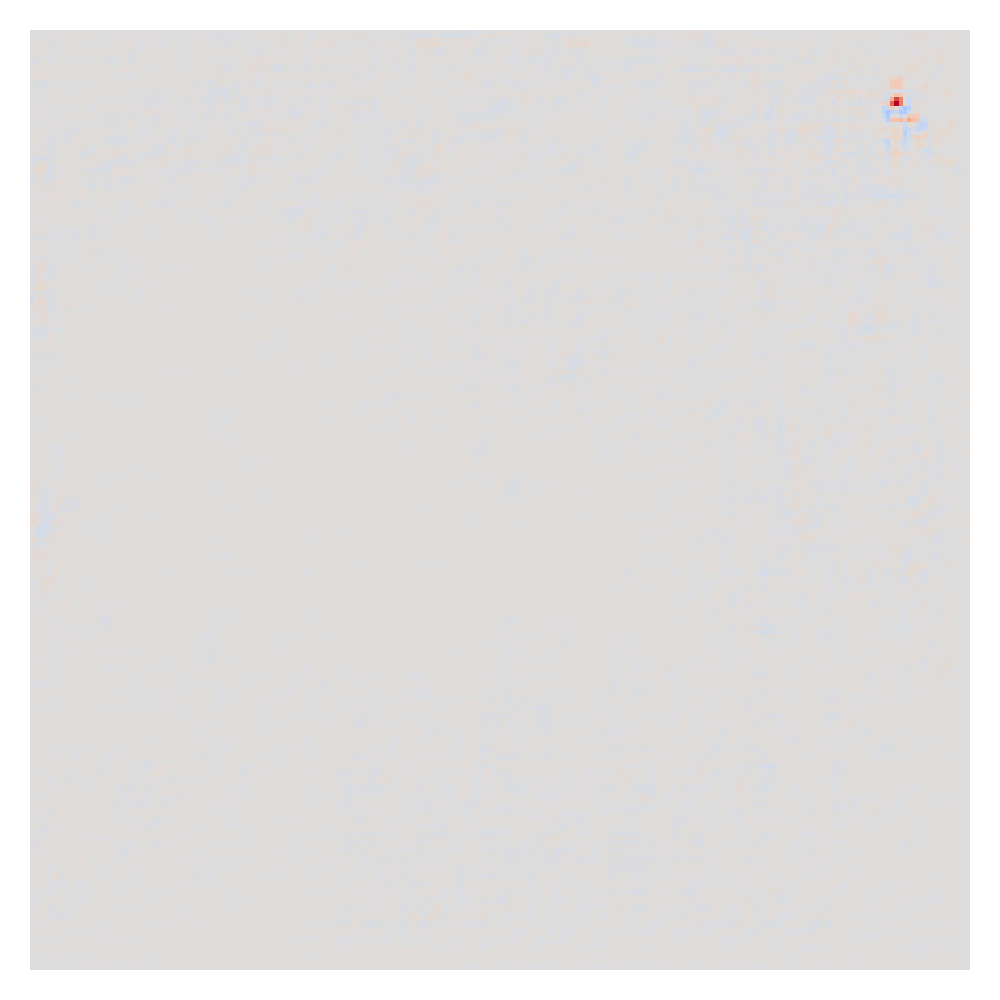
\includegraphics[height=1\linewidth]{01-images/05-resultate/uap_resnet50/uap0-resnet50-covidx_data-n200-robustificationslevel0.png}
        \caption{ResNet50\\\textcolor{white}{Despotar}}
    \end{subfigure}
    \caption{Darstellung generierter \acrshort{uap}s für den COVIDx CXR-4-Datensatz, basierend auf 200 Trainingsbildern und verschiedenen Klassifikationsmodellen.}
    \label{fig:unterschiedliche-uaps-covid}
\end{figure}

Analog wie bei Abbildung \ref{fig:unterschiedliche-uaps-mri} werden die Perturbationen auf dem COVIDx CXR-4 Datensatz trainierten Modelle visualisiert.

Bei der \acrshort{uap} von DenseNet121 sind die Perturbationen im oberen rechten Bereich des Bildes stärker ausgeprägt, während sie im restlichen Bildbereich gleichmässig verteilt sind. Es treten punktuelle Perturbationen mit hohen Werten auf, die eine erhöhte Sensitivität des Modells in diesen Bereichen anzeigen. Im Gegensatz dazu zeigt die \acrshort{uap} für DenseNet169 eine gleichmässige Verteilung der Perturbationen über das gesamte Bild. Eine auffällige, intensive, rote Stelle im oberen rechten Bereich weist auf eine spezifische Schwäche hin. Bemerkenswert ist, dass bei DenseNet169 nur ein intensiver roter Punkt existiert, während bei DenseNet121 mehrere solcher Punkte in der gleichen Region vorhanden sind.

Die \acrshort{uap} für EfficientNetV2-S weist horizontale Muster auf, die über die gesamte Heatmap gleichmässig verteilt sind. Ein ähnliches Muster, das bei Abbildung \ref{fig:uap-densenet121-mri-prerobustification} beobachtet wurde. Im Gegensatz dazu weist das grössere Modell, EfficientNetV2-M, auffällige vertikale Linien im oberen linken und unteren mittleren Bereich der \acrshort{uap} auf. Im Zentrum sind rote Bereiche erkennbar, die von blauen Flächen links und rechts eingerahmt werden. Zudem sind zwei grosse blaue Flecken auf der rechten Seite sichtbar.

Die \acrshort{uap} für ResNet18 zeigt ein diagonales, wellenförmiges Muster. Diese Struktur ist über die gesamte \acrshort{uap} hinweg sichtbar. Auffällig ist die hohe Konzentration von solchen Perturbationen auf der rechten Seite und in der oberen rechten Ecke, wobei sowohl hohe rote als auch blaue Werte nebeneinander auftreten. Im Vergleich dazu zeigt die \acrshort{uap} für ResNet50, wie beim DenseNet169, lediglich in der oberen rechten Ecke einen starken Ausschlag. Ansonsten bleibt die Verteilung der Perturbationen über das gesamte Bild hinweg gleichmässig und fein.

\newpage